% file: 3-6-graph-decomposition/bicomponent-example-graph.tex

\documentclass[tikz]{standalone}
\usetikzlibrary{positioning}

\begin{document}
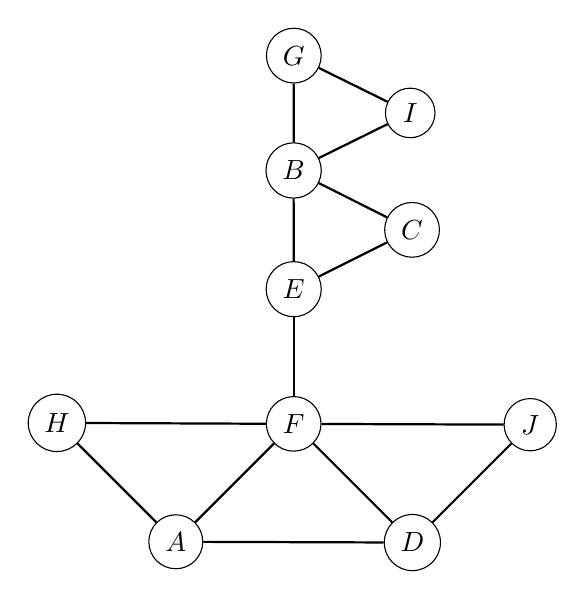
\begin{tikzpicture}[every node/.style = {draw, circle, minimum size = 6pt},
  node distance = 0.25cm and 1.0cm,
  every edge/.style = {draw, thick}]
  \node (g) {$G$};
  \node (i) [below right = of g] {$I$};
  \node (b) [below left = of i] {$B$};

  \node (c) [below right = of b] {$C$};
  \node (e) [below left = of c] {$E$};

  \begin{scope}[node distance = 1.00cm and 1.0cm]
    \node (f) [below = of e] {$F$};
    \node (a) [below left = of f] {$A$};
    \node (d) [below right = of f] {$D$};
    \node (h) [above left = of a] {$H$};
    \node (j) [above right = of d] {$J$};
  \end{scope}

  \path (g) edge (b)
  	    edge (i)
  	(b) edge (e)
  	    edge (i)
  	    edge (c)
	(e) edge (f)
  	    edge (c)
	(f) edge (h)
	    edge (a)
	    edge (d)
	(h) edge (a)
	(a) edge (d)
	(d) edge (j)
	(j) edge (f);
\end{tikzpicture}
\end{document}